\section{Ejercicio 2 (BackTracking con Poda):}

En este ejercicio nos piden hacer una mejora en el anterior algoritmo de backtracking y hacerle una poda. Las podas consisten en que hay instancias de soluciones parciales que ya no nos interesan y ni siquiera las necesitamos calcular, porque por ejemplo esta solución va a hacer peor que una que ya calculamos anteriormente. Esto lo que provoca es una optimización porque dejamos de calcular cosas, aunque sigue siendo una búsqueda exhaustiva, si vemos las el árbol de recursión lo que pasa es que cortamos muchas ramas.

Si recordamos el anterior algoritmo, para un índice calculaba el menor si lo pintamos de rojo, despues de azul y después sin pintar, pero que pasa si uno nos devuelve que se pueden pintar todos los proximos numeros, osea que los los otros no hace falta computarlos ya que solo nos importa la cantidad de números sin pintar, y no vamos a encontrar una mejor porque esta es la mínima. Esta es nuestra primer poda, una vez calculado una solución parcial para un color, nos fijamos si es óptima y si lo es nos salteamos(no computamos) las otras alternativas de colores.	

Tambien podriamos llevar una cuenta de cuál es la solución(entera) óptima y no calculamos una que pueda ser peor que esa, por ejemplo si voy por el 3 índice y encontramos una solución que solo no puede pintar un numero, solo tenemos que buscar una solución que pinta todos los numeros, asi que no vamos a entrar a las recursiones de no pintar.

Para la implementación de estas podas modificamos un poco la base del código del anterior ejercicio así se nos es más fácil calcular los datos. Ahora la función recursiva tiene 2 parámetros de entrada nuevos, el mínimo encontrado en las soluciones ya calculadas(lo pasamos por referencia y editamos ese) y la cantidad de números que ya no pintamos y ahora en vez de devolver un resultado parcial, devuelve la cantidad de  números sin pintar para todo el arreglo(ya que tenemos la cantidad que no pintamos antes).

Podemos afirmar que el algoritmo sigue siendo correcto porque las únicas subsoluciones que descartamos son las que ya sabemos que no van a ser las óptimas, esta es la gracia de la poda en el backtracking.

\subsection*{Pseudocodigo}
\begin{algorithm}[H]
\NoCaptionOfAlgo
	\KwData{	
	arreglo = el arreglo de numeros entero\\
	n = el tamaño del arreglo
	\KwResult{La cantidad minima de numeros sin pintar para una secuencia de numeros de largo n}
	\caption{\algoritmo{ej2}{int arreglo[], n}{int}}
		\tcc{Empezamos el backtracking desde el primer indice(0) y no inicializamos todavia el ultimo rojo y el ultimo azul, y ademas por defecto el optimo es n(no existe peor solucion que esta) y no pintamos ninguno todavia}
		res $\leftarrow$ BT(0, arreglo, n, NULL, NULL, n, 0)\\
	}
\end{algorithm}
.\\
\begin{algorithm}[H]
	\NoCaptionOfAlgo
	\KwData{
	i = indice actual a pintar\\
	arreglo = el arreglo de numeros entero\\
	n = el tamaño del arreglo\\
	ultimoRojo = el ultimo numero que se pinto de rojo(NULL si no se pinto ninguno)}
	ultimoAzul = el ultimo azul pintado\\
	optimoActual = la mejor solucion encontrada hasta el momento
	sinPintar = cantidad de numeros sin pintar antes de i\\
	\KwResult{La cantidad minima de numeros sin pintar a partir de i hasta n}
	\caption{\algoritmo{BTI}{int i, arreglo[], n, ultimoRojo, ultimoAzul, optimoActual, sinPintar}{int}}

	numeroActual $\leftarrow$ arreglo[i]\\
	\eIf{ i = $n-1$ }{
		\tcc{Si el indice es el ultimo numero entonces estamos en el caso base}
		\tcc{Tenemos que fijarnos si podemos pintarlo}
		\eIf { ultimoRojo = NULL \textbf{or} ultimoAzul = NULL \textbf{or} ultimoRojo $<$ numeroActual \textbf{or} ultimoAzul $>$ numeroActual }{
			res  $\leftarrow$ sinPintar
		}{
			\tcc{No lo podemos pintar porque no seria una solucion valida entonces devolvemos la cantidad que pintamos antes mas 1 porque este no lo pintamos}
			res  $\leftarrow$ sinPintar + 1
		}
	}{	
		int minSiRojo, minSiAzul, minSinPintar\\
		\If{ ultimoRojo = NULL \textbf{or} ultimoRojo $<$ numeroActual} {
			minSiRojo $\leftarrow$ BTI(i+1, arreglo, n, numeroActual, ultimoAzul, optimoActual, sinPintar)\\
			\tcc{PODA 1: si es el optimo no calculamos los demas y devolvemos este}
			\If{minSiRojo $=$ sinPintar}{
				res $\leftarrow$ minSiRojo
			}
			\If{ minSiRojo $<$ sinPintar} {
				optimoActual $\leftarrow$ minSiRojo
			}
		}
		\If{ ultimoAzul = NULL \textbf{or} numeroActual $<$ ultimoAzul} {
			\tcc{Lo mismo con el azul}
			minSiAzul $\leftarrow$ BTI(i+1, arreglo, n, ultimoRojo, numeroActual, optimoActual, sinPintar)\\
			\tcc{PODA 1}
			\If{minSiAzul $=$ sinPintar}{
				res $\leftarrow$ minSiAzul
			}
			\If{ minSiAzul $<$ sinPintar} {
				optimoActual $\leftarrow$ minSiAzul
			}
		}
		\tcc{PODA 2: solo calculamos sin pintar este numero, si todavia podemos mejorar el optimo}
		\If{sinPintar $<$ optimoActual $- 1$} {
			minSinPintar $\leftarrow$ BTI(i+1, arreglo, n, ultimoRojo, ultimoAzul, optimoActual, sinPintar + 1)\\
		}
		res $\leftarrow$ min(minSiRojo, minSiAzul, minSinPintar)
	}

\end{algorithm}

\subsection*{Análisis de Complejidad}
La cantidad de recursiones a la que se sigue podiendo entrar sigue siendo de 3, osea que sigue siendo $O(3^n)$, si bien va a disminuir demasiado las recursiones que hacemos(ya que con estas podas cortamos muchos caminos), esto va a mejorar muchos el promedio de los casos, en los que casi siempre vamos a cortar muchas ramas. El mejor caso ahora es lineal, si nos dan una secuencia creciente, la primer solución que se encuentra es la que pintamos todos de rojo y como es 0 ya devolvemos eso, esto es $O(n)$ 

\subsection*{Experimentación Computacional}
\subsubsection*{Instancias Aleatorias}
Se corrieron la experimentacion sobre la misma computadora y para los mismos arreglos que para el anterior ejercicio
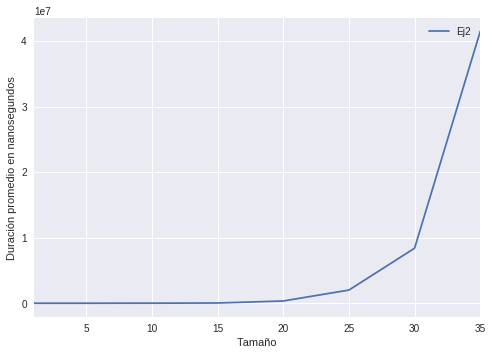
\includegraphics[scale=0.5]{ej2Random1-40.png}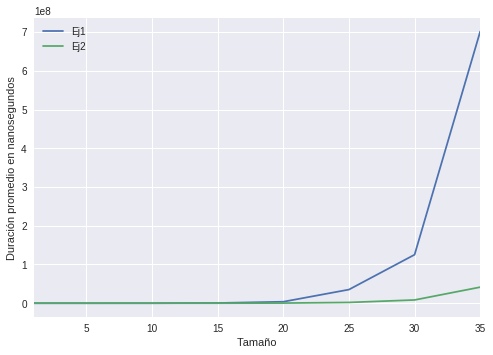
\includegraphics[scale=0.5]{ej12Random1-40.png}\\
A simple vista podemos ver que sigue creciendo exponencialmente, pero al compararlo con el algoritmo de sin poda notamos una gran mejora. Para instancias de 35 el original tarda 0,701732075 segundos pero el nuevo tarda 0,041461628 segundos 16 veces menos. Estos tiempos ya son mas viables que el anterior ejercicio.

   




